The methods used in this study follow those of the framework presented in \cite{ramirezgomezTechnoeconomicGISbasedModel2018}, with some key additions and improvements. The summary of the methodology and methods is presented in \fref{fig:framework}.

\begin{figure*}[!h]
	\centering
	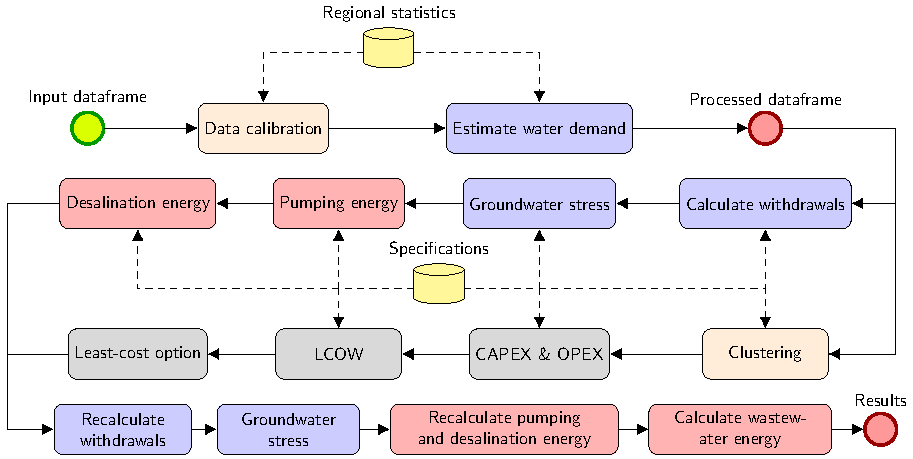
\includegraphics[width=\textwidth]{Framework}
	\caption{Methodology flow diagram---blue boxes indicate water-related methods, red boxes energy-related methods, gray boxes cost and LCOW related methods, orange boxes supporting methods and the yellow cylinders scenario characteristics data.}
	\label{fig:framework}
\end{figure*}

The water-agriculture-energy system evaluated for the NWSAS consisted of the extraction of groundwater resources, desalination of brackish water when needed, water demand for domestic and agricultural irrigation purposes, reclaim of domestic wastewater and agricultural drainage (i.e. tailwater), treatment of reclaimed wastewater, and treated wastewater reuse in agricultural irrigation. A schematic of the system is presented in \fref{fig:system_reuse}.

\begin{figure*}[!h]
	\centering
	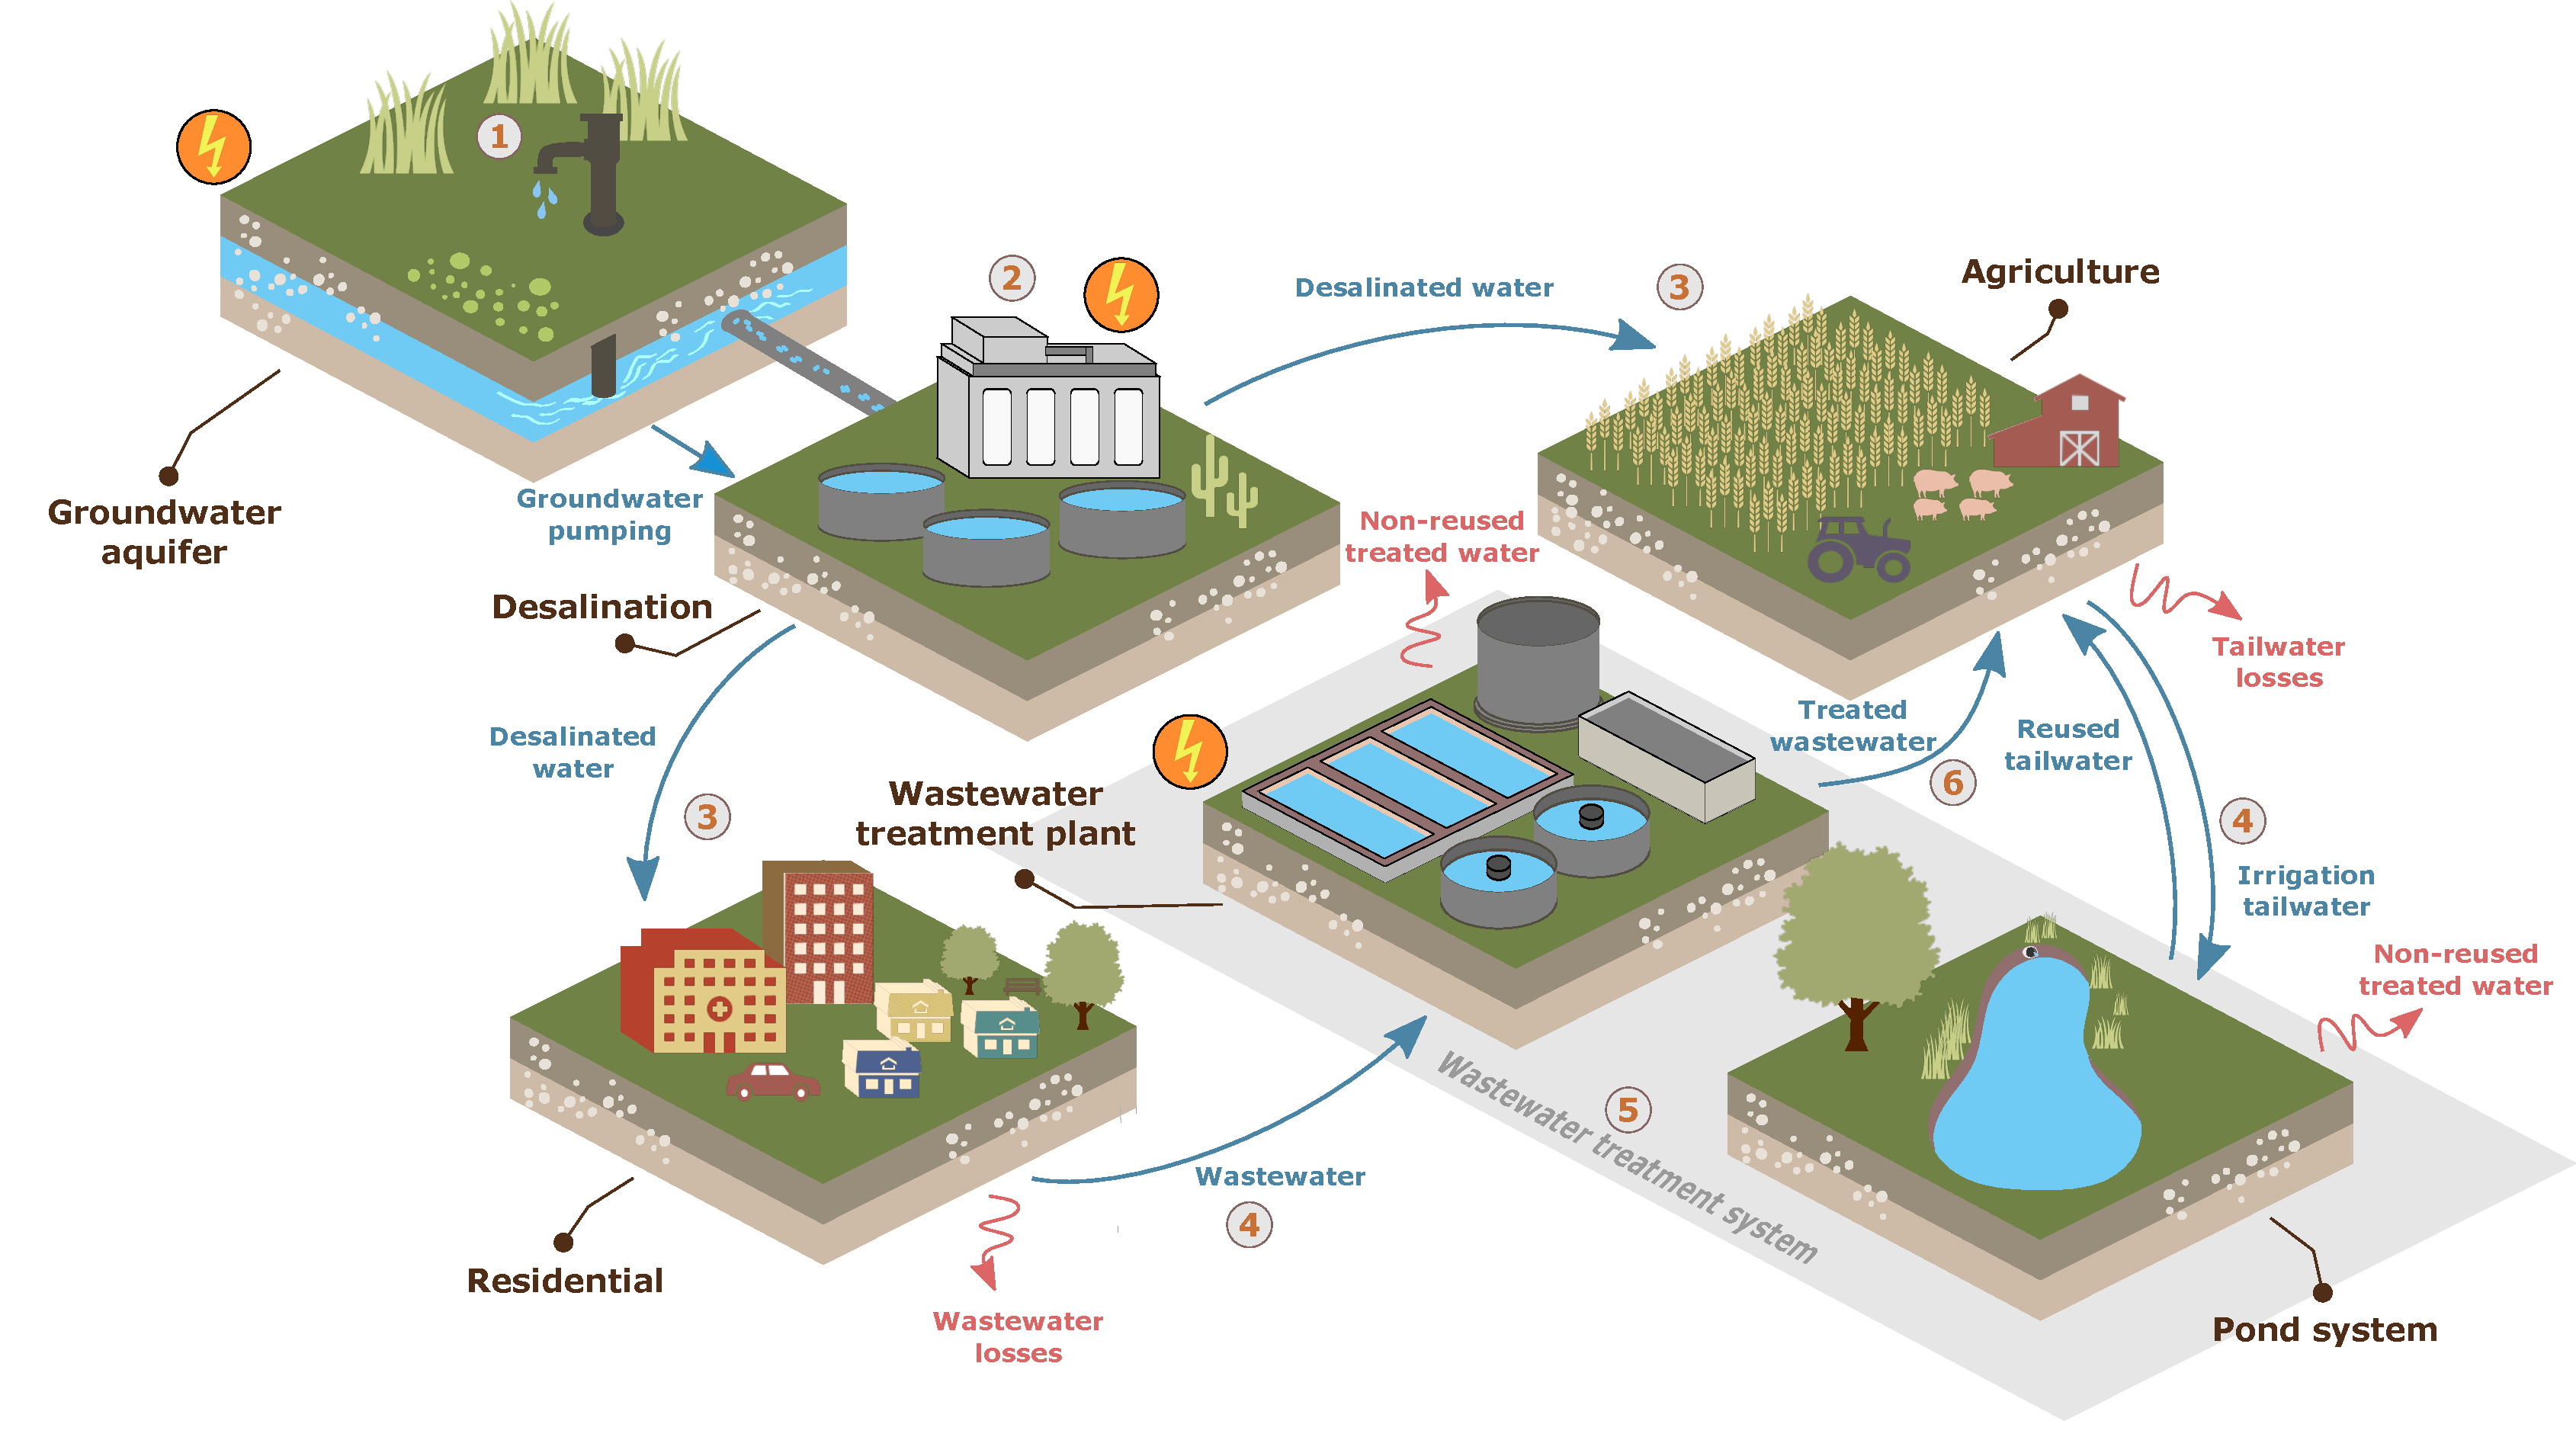
\includegraphics[width=\textwidth]{System_reuse}
	\caption{NWSAS components and resource streamflows - WWR scenarios.}
	\label{fig:system_reuse}
\end{figure*}

All water requirements for population consumption and agricultural irrigation were assumed to be supplied by the groundwater aquifer and that such water is desalinated whenever the TDS levels are above 1,000 mg/l \cite{fao1985water}. Afterwards, the water is allocated for population consumption and agricultural irrigation. 
% Finally, wastewater from population and tailwater from agriculture is disposed to the environment without any adequate treatment. 
The recharge rate $R$ for the entire aquifer was taken as 1.1 billion cubic meters of water per year, which for the area of the aquifer, is an equivalent water column of 1.06 mm per year \cite{BetterValorizationIrrigation2015}. Furthermore, no environmental flow was considered.

Six wastewater treatment and reuse scenarios were analysed, evaluating three irrigation water pricing regimes and two levels of population water consumption. Irrigation water pricing regimes were taken from \cite{Socioeconomicaspectsirrigation2014}, were it was found that the irrigation water demand per hectare throughout the NWSAS basin is heavily dependent on the supply water cost. Three different regimes for water users exist: 

\begin{enumerate}
	\item \textbf{Private water users:} private farmers that pay the full price of water without any subsidy. The average level of water demand is around 10,512 m\textsuperscript{3}/ha. The \citet{Socioeconomicaspectsirrigation2014} found, that farmers belonging to this regime, have higher water productivity. 
% 	This means that, they have a better use of the resource, obtaining more product while using less amount of irrigation water per hectare.
	\item \textbf{Subsidized water users:} users that have access to water subsidized to some extent. The average water demand is 15,334 m\textsuperscript{3}/ha.
	\item \textbf{Free water users:} farmers that have free access to water, meaning that the government fully subsidize the price of water and that the resource can be utilized without limitations. The average irrigation water demand is 21,215 m\textsuperscript{3}/ha.
\end{enumerate}

Water demand in the subsidized and free regimes, constitutes a 45.8\% and a 101.8\% increase in irrigation water requirements compared to the private regime respectively. This suggests a strong price elasticity of the irrigation water demand and/or the use of lower efficiency irrigation technologies \cite{Socioeconomicaspectsirrigation2014}.

On the other hand, two levels of population water consumption were analysed based on the work of \citet{Householdwaterconsumption2014}:

\begin{enumerate}
    \item \textbf{Low level:} an average water consumption per capita of 55 m\textsuperscript{3}/year.
    \item \textbf{High level:} an average water consumption per capita of 73 m\textsuperscript{3}/year.
\end{enumerate}

In addition, a sensitivity analysis was performed on the groundwater quality and depth to groundwater levels, in order to asses the impact they pose to the energy-for-water requirements (\tref{tbl:sensitivy}). This parameters were selected, as the water security of the aquifer highly depends on the water table levels and the quality of the resource, directly affecting food security as well.

\begin{table}[!ht]
	\caption{\label{tbl:sensitivy}Sensitivity parameters.}
	\begin{indented}
	\item[]\begin{tabular}{@{}l l l l}
		\br
		Parameter & Low & middle & high\\
		\mr
		Groundwater quality & -10 meters & current level & +10 meters\\
		Depth to groundwater & -50\% & current level & +50\%\\
		\br
	\end{tabular}
	\end{indented}
\end{table}

% \noindent Groundwater quality:
% \begin{itemize}
% 	\item Low: -50\% of the current TDS levels,
% 	\item Neutral: the current TDS levels,
% 	\item High: +50\% of the current TDS levels.
% \end{itemize}

% \textbf{Depth to groundwater:}
% \begin{itemize}
% 	\item Low: -10 meters of the current depth to groundwater levels,
% 	\item Neutral: the current depth to groundwater levels,
% 	\item High: +10 meters of the current depth to groundwater levels.
% \end{itemize}

% \subsection{Geographic Information Systems analysis}

% \begin{table*}[b]
% 	\caption{\label{tbl:datasources}Geographic Information System data sources}
%     {\footnotesize
%     \begin{tabular*}{\textwidth}{@{}P{1.4in} P{1in} l P{1.2in} l l@{}}
%     \br
%     Layer & Coverage & Format & Resolution & Year & Source\\
%     \mr
%     Population & Algeria, Tunisia, Libya & raster (tif) & 100 m grid cell & 2015 & \cite{Worldpop2012}\\\ms
%     Depth to groundwater & Africa & txt table & 5 km grid cell & 2012 & \cite{Quantitativemapsgroundwater2012a}\\\ms
%     Administrative boundaries & Africa & shapefile & Individual country polygons & 2017 & \cite{Humanitarian2017}\\\ms
%     Administrative boundaries & Algeria, Tunisia, Libya & shapefile & Level 1 (provinces) polygons & 2015 & \cite{GADM}\\\ms
%     Transboundary aquifers borders & Global & shapefile & Individual polygons & 2015 & \cite{IGRAC}\\\ms
%     Groundwater quality & NWSAS Basin & data points & 206 data points & 2016 & RA*\\\ms
%     Digital Elevation Data* & Africa & raster (tif) & 1, 3 and 15 arc second & 2014 & \cite{DEM2014}\\\ms
%     Land cover & Africa & raster (tif) & 20 m grid cell & 2016 & \cite{ESA2017}\\\ms
%     Aquifer boundaries & NWSAS basin & shapefile & Individual polygons & - & RA*\\\ms
%     Climate data & Global & raster (tif) & 30 arc second, monthly & 1970-2000 & \cite{WorldClimGlobalClimate}\\
%     \br
%     \end{tabular*}\\
%     ~* Regional Authorities.
%     }
% \end{table*}

The most up-to-date open source data available was collected and processed using the open source Geographic Information System software QGIS. A data package comprising the geospatial characteristics of the study area was created, in order to capture key information to make the WEF nexus analysis possible. The relevant layers are identified and described in \tref{tbl:datasources}.

% All data layers were converted into matching units, re-projected into the Sud Algerie Degree projection (ESRI: 102592)---This projection was selected as it produces minimal distortions in the analysis area---, re-scaled to the same resolution and, when only individual data points were available, interpolated to extend the data to the entire analysed area (i.e. for the Groundwater quality layer). Furthermore, all layers were merged into a large data frame.

% \subsection{Data calibration}
% The \textit{population} and the \textit{irrigated area} layers were calibrated to match regional statistics. The calibration was performed using the fraction given between the regional statistical data (i.e. total population or total irrigated area), and the sum of all data points of the layer in question. The statistical data was available as per country basis. Thus, the calibration process was performed for the basin areas within each country, using their specific information (see \tref{tbl:regionalstats}).

% \begin{table*}[!h]
% 	\caption{\label{tbl:regionalstats}NWSAS population and irrigated area statistics for year 2015, subdivided per country area inside the basin. Data source: \cite{BetterValorizationIrrigation2015}}
% 	\begin{indented}
% 	\item[]\begin{tabular}{@{}l*{4}{r}}
% 		\br
% 		Parameter & Total & Algeria & Tunisia & Libya\\
% 		\mr
% 		NWSAS Population & 6,376,367 & 4,240,888 & 617,168 & 1,518,311\\
% 		NWSAS Irrigated area (Ha) & 469,529 & 237,485 & 56,547 & 175,497\\
% 		\br
% 	\end{tabular}
% 	\end{indented}
% \end{table*}

% Moreover, to calibrate the irrigated area data, an algorithm was run to ensure that non of the data cells had more than 100\% of its area covered by irrigated land.
 
% \subsection{Population and irrigation water withdrawals}
% The calculation of total water withdrawals $ww_{tot,i}$ was performed according to \eref{eq:waterwithdrawals}. Population water withdrawals were calculated as the product between the population count in each data cell ($Pop_{i}$) and the specific water demand per capita ($wpc_{i}$) for the region. Similarly, withdrawals from irrigated agriculture were calculated as the product between the irrigated area inside each data cell ($IrrArea_{i}$) and the specific water demand per cultivated hectare ($wpha_{i}$) for the region.

% \begin{equation}\label{eq:waterwithdrawals} 
% ww_{tot,i} = Pop_{i}\cdot wpc_{i} +IrrArea_{i}\cdot wpha_{i} 
% \end{equation}

% For the baseline, a level of water withdrawals per capita $wpc$ of 55 cubic meters per year was assumed with a population growth of 1\% per year \cite{Householdwaterconsumption2014}. Moreover, all cropland area within the aquifer was considered to be irrigated by groundwater resources and the water requirements per cultivated hectare $wpha$ to be 13,520 m\textsuperscript{3}/Ha for the Algerian part; 13,266 m\textsuperscript{3}/Ha for Tunisia and 9,134 m\textsuperscript{3}/Ha for Libya, according to data from \cite{Socioeconomicaspectsirrigation2014}. Finally, no growth in irrigated area was considered.

\subsection{Reclaimed wastewater and reused treated wastewater}
The amount of residential recoverable wastewater, was assumed to represent around 70\% of the total residential water consumed \cite{unescoWastewaterUntappedResource2017}. From that share, an additional 10\% was assumed to be lost in the capture, conveyance and treatment processes.
On the other hand, to evaluate the potential of capturing, storing and reusing irrigation tailwater, first the water requirements of the crop were estimated. The FAO-56 Penman-Monteith method \cite{allenFAOIrrigationDrainage1998} was used, calculating meteorological parameters from ``WorldClim" monthly data \cite{WorldClimGlobalClimate} through the Python library ``Pyeto" \cite{pyeto}. For the purpose of this study, date palms were assumed to cover 100\% of the cropland area---as is one of the main crops cultivated in the region. The crop coefficients and irrigation calendar were set according to \citet{almullaNWSAS}. From this process, the yearly crop water needs throughout the entire basin were obtained.

Furthermore, an on-farm storage pond system was evaluated to account for the potential reusable water. For this, a water balance on the on-farm storage was executed following a similar approach to \citet{reinhartSimulatedWaterQuality2019}. First, the maximum irrigation efficiency (i.e. crop water requirements over irrigation water needed) was set to be 80\%, being the remaining 20\% non-recoverable loses. If additional water was available, it was recovered and stored. The storage reservoir surface area, was assumed at 2\% of the cropland area and a standard depth of 3 meters \cite{reinhartSimulatedWaterQuality2019}. Leakage losses in the storage system were set to be 0.9 mm/day, and evaporation loses were calculated using a modified Penman-Monteith method for an open water body \cite{reinhartSimulatedWaterQuality2019}. For this, and albedo, surface height, and surface roughness values of 0.05, 0.002 m, and 0 s/m, respectively were used \cite{princeczarneckijobym.QuantifyingCaptureUse2017}.

\subsection{Groundwater Stress Indicator}
The Groundwater Stress Indicator was used to quantify the current stress of the aquifer \cite{Aqueductglobalmaps2015}. It relates the ratio of water withdrawals due to anthropogenic reasons (e.g. potable water, industrial water, recreational water, irrigation water, etc.), and the total recharge rate of the aquifer (subtracting the environmental stream flow). The groundwater stress indicator is usually calculated as the ratio of groundwater footprint to aquifer area \cite{RegionalGroundwaterStress2013}.

% as per \eref{eq:7}:

% \begin{equation}\label{eq:7} 
% GW = \frac{GF}{A_{A}}
% \end{equation}

% \noindent{Where}:
% \begin{itemize}[label={-}]
% 	\item $GW$: Groundwater Stress indicator. Values below 1 indicate low stress areas, values from 1 to 5 indicate low to middle stressed areas, values from 5 to 10 indicate middle to high stressed areas, values from 10 to 20 indicate high stressed areas and values above 20 indicate extremely high stressed areas.
% 	\item $GF$: groundwater footprint. Identifies the right balance between groundwater use and groundwater replenishment for an area.
% 	\item $A_A$: areal extent of an aquifer throughout a given region.
% \end{itemize}

% The groundwater footprint is calculated as:

% \begin{equation}\label{eq:8} 
% GF = \frac{C}{R-E}\cdot A
% \end{equation}

% \noindent{Where}:
% \begin{itemize}[label={-}]
% 	\item $C$: total area-averaged annual withdrawals of groundwater for anthropogenic use.
% 	\item $R$: total area-averaged annual recharge rate of water for groundwater aquifer, including natural and anthropogenic sources.
% 	\item $E$: total area-averaged annual environmental stream flow used to sustain ecosystem services.
% 	\item $A$: areal extent of a given region where $C$, $R$, and $E$ can be defined.
% \end{itemize}

% \subsection{Groundwater pumping}\label{Sc:pumping}
% The energy needs to pump water from groundwater resources is given by the required lift ($H-h$), the pressure drop due to fluid friction in the piping, and the pressure losses in valves and fittings. Pressure losses due to friction in the piping were found to be rather small compared to the lift requirements. Therefore, and due to lack of specific data on wells and boreholes in the region, the pressure losses due to friction in the piping and in valves and fittings were disregarded. The energy requirements (in watt-h) can then be estimated as \eref{eq:1} \cite{Groundwaterdependentirrigationcosts2017}:

% \begin{equation}\label{eq:1}
% E = \frac{Q\cdot(\rho\cdot g\cdot(H - h))}{\eta}
% \end{equation}

% Where $Q$ stands for the water extractions (m\textsuperscript{3}), $\rho$ for the water density (kg/m\textsuperscript{3}), $g$ for the gravitational acceleration (m/s\textsuperscript{2}), $H$ for the delivered hydraulic head (meters), and $h$ for the head in the well (meters). Moreover, $\eta$ accounts for the pumping efficiency, which was set as 85\% along the entire aquifer.

% \subsection{Reverse Osmosis desalination}\label{Sc:RO}
% Reverse Osmosis (RO) desalination is the most popular desalination technology used worldwide. Its energy intensity falls typically in the range of 0.5 to 2.5 kWh per cubic meter of desalinated brackish water \cite{Energyoptimalgroundwater2013}.

% To estimate the energy required to desalinate one cubic meter of saline water, often detailed information of the RO system is required. When analysing a broad area using a geospatial approach, such information is not available as the characteristics of the system can change from application to application \cite{stillwellPredictingSpecificEnergy2016,aminfardMultilayeredSpatialMethodology2019}. Thus, a simplified approach was used to estimate the RO energy requirements. RO is a pressure-driven process that forces water through a membrane which separates dissolved solutes using preferential diffusion. The output water from the membrane (\textit{permeate, p}) is relatively free of solutes, while the remaining water (\textit{concentrate, c}) exits the pressure vessel with a high concentration of solutes (i.e. high TDS levels). A schematic representation of the process is presented in \fref{fig:ro} \cite{crittenden_mwhs_2012}.

% \begin{figure}[!ht]
% 	\centering
% 	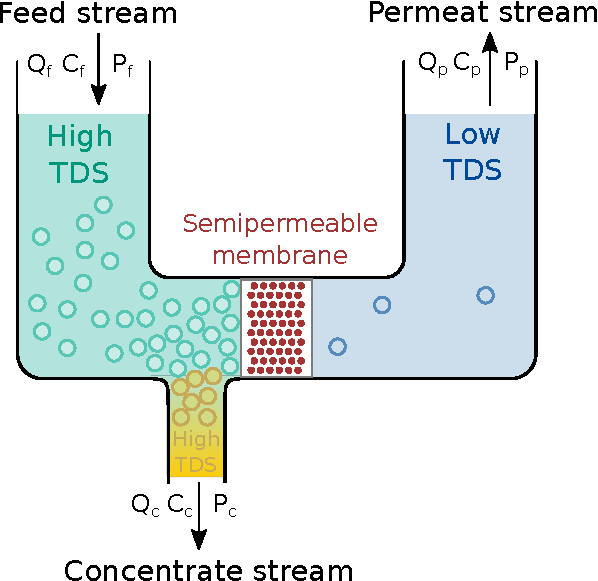
\includegraphics[width=0.4\textwidth]{Reverse_Osmosis}
% 	\caption[Reverse Osmosis schematic separation process]{Reverse osmosis schematic separation process. Based on: \cite{crittenden_mwhs_2012}.}
% 	\label{fig:ro}
% \end{figure} 

% The minimum energy required to push the water through the membrane is given by the amount of diluted solutes in the \textit{feed (f)} water. Such minimum energy can be estimated calculating the osmotic pressure of the \textit{feed} water, as described in \eref{eq:6} \cite{crittenden_mwhs_2012}.

% \begin{equation}\label{eq:6}
% \pi = \phi\cdot C\cdot R\cdot T
% \end{equation}

% \noindent{Where}:
% \begin{itemize}[label={-}]
% 	\item $\pi$: osmotic pressure (bar),
% 	\item $\phi$: osmotic coefficient, close to 1 (-), assumed a 0.95 \cite{crittenden_mwhs_2012},
% 	\item $C$: concentration of all solutes (mol/L),
% 	\item $R$: universal gas constant, 0.083145 (L$\cdot$bar/mol$\cdot$K),
% 	\item $T$: absolute temperature (K), (273 + \degree C), assumed at 25 \degree C for the entire aquifer.
% \end{itemize}

% Thus, the minimum energy demand can be estimated multiplying the osmotic pressure of the \textit{feed} water $\pi$ (in bar) by a conversion factor of 1.0 kWh/m\textsuperscript{3} = 36 bar. In reality, the energy demanded is greater due to factors as friction losses, membrane filtration resistance, among others. However, this approach has been used in cases were no specific data of the RO system is available \cite{KARABELAS201815}.

% The water quality layer used, was obtained from 206 measurements provided by National Authorities of the region. Each point specifies the spacial location and groundwater TDS content. Although the data did not covered the entire basin area, due to lack of any other related information it was used to produced a raster layer. An inverse distance weighted interpolation method, having as distance weighting factor an inverse distance to a power of 2 and a global search radius with maximum number of nearest points of 10 was used (see \fref{fig:TDS}).

% \begin{figure*}[!ht]
% 	\centering
% 	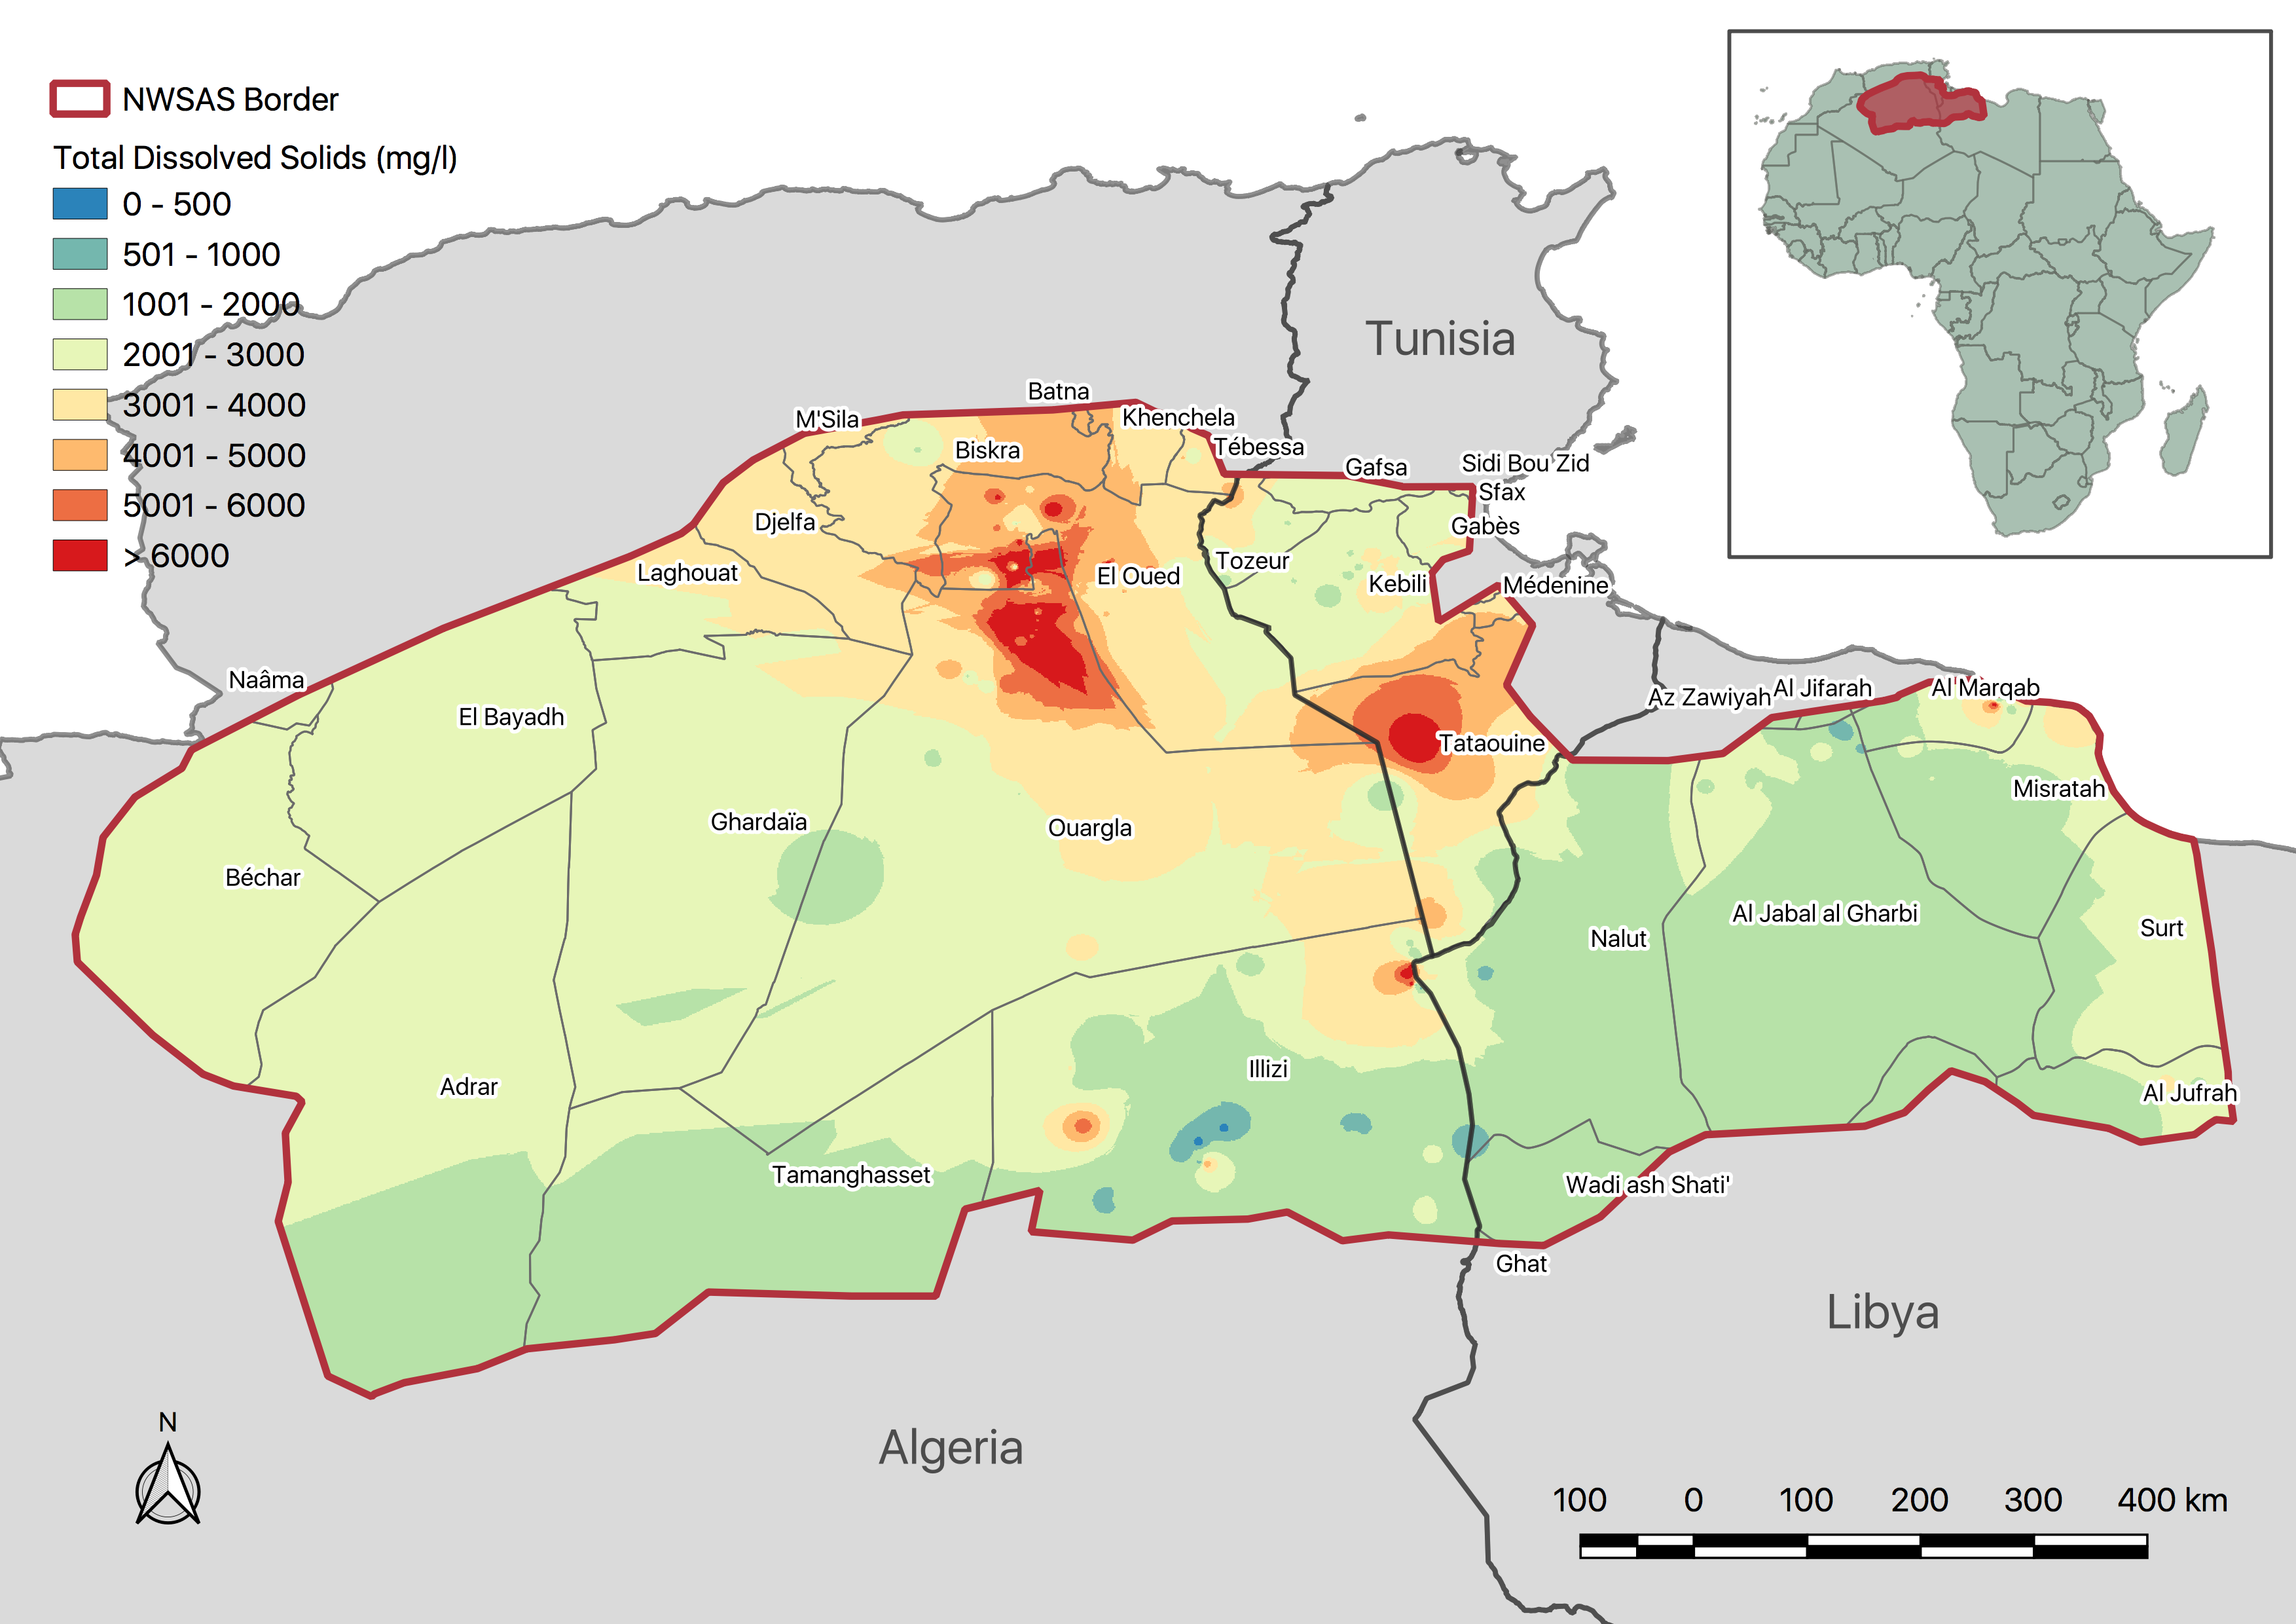
\includegraphics[width=0.88\textwidth, cfbox=black 1pt 0pt]{NWSAS_TDS}
% 	\caption[NWSAS groundwater quality map - Total Dissolved Solids (TDS)]{North Western Sahara Aquifer System - Groundwater quality map, Total Dissolved Solids (TDS) at 1$\times$1 km grid cell resolution.}
% 	\label{fig:TDS}
% \end{figure*}

% \subsection{Energy-for-wastewater}\label{Sc:eww}
% To calculate the energy-for-wastewater requirements an energy intensity factor was used for each evaluated treatment technology following \eref{eq:energy-for-wastewater}.

% \begin{equation}\label{eq:energy-for-wastewater}
% E_{ww} = Q_{ww,yr}\cdot X_t
% \end{equation}

% Where $Q_{ww,yr}$ represents the yearly treated wastewater in m\textsuperscript{3}/yr, and $X_t$ the average energy demand of the specific WWTT $t$, to treat one m\textsuperscript{3} of wastewater (in kWh/m\textsuperscript{3}).

\subsection{Clustering algorithm}\label{Sc:clustering}
A clustering approach was used in order to identify dense areas where a WWTS could be implemented, minimizing constraints imposed by existent large distances among scatter population or irrigated lands. A hierarchical clustering  algorithm was run using the \textit{Agglomerative Clustering} object from the Python \textit{scikit-learn} package \cite{scikit-learn}.
% Such algorithm relies on a bottom-up approach to define the clusters, in which all data points are first identified as an individual cluster, to be then successively merged together. The linkage criteria used was the \textit{ward} linkage.

\subsection{Wastewater Treatment System characteristics}
% The costs incurred in the implementation of a WWTS, can be divided into three major groups: \begin{enumerate*}[label=\upshape(\arabic*\upshape)]
% 	\item CAPEX, \item OPEX and \item Conveyance or transport system costs.
% \end{enumerate*} The first two, account for capital and operation expenses, and the third one for implementation and operation of the wastewater transportation system. Due to the high complexity of evaluating the costs of a conveyance system, only CAPEX and OPEX costs were considered.

% Statistical methods have shown to be commonly used among cost-modelling for wastewater management \cite{Costmodellingwastewater2011,Assessmentwastewatertreatment2012,Economicfeasibility2012}. Such methods use available cost figures (i.e. historical or estimated cost figures of actual WWTPs as capacity, pollutants treated, etc.) to create cost functions that adjust the cost relevant data to independent variables, describing the behaviour of a dependent variable (i.e. CAPEX and OPEX). The resulting cost function, allows to evaluate the capital and operational costs, often in terms of wastewater flow or served population equivalent \cite{Economicvaluationwastewater2015}. One advantage of this approach from a GIS perspective, is that with the use of non-linear cost functions, the effect of economies of scale can be easily evaluated. Furthermore, as a top-down approach enables for a better understanding of the relationship among variables and wastewater management, it constitutes a scientific approach for new wastewater services planning \cite{Costmodellingwastewater2011}. 

Wastewater pollutant levels, were assumed to be constant throughout the basin, using standard values based on studies from FAO \cite{fao1985water}. The assumed pollutant levels for population wastewater and the required levels for reused TWW, are shown in \tref{tbl:pollutans}.

% \begin{table*}[!ht]
% 	\caption{\label{tbl:pollutans}Pollutant levels of wastewater and treated wastewater (mg/l).}
% 	\begin{indented}
% 	\item[]\begin{tabular}{@{}l r r}
% 		\br
% 		Pollutant type & Wastewater & Treated wastewater\\
% 		\mr
% 		Suspended solids ($SS$) & 900 & 100\\
% 		Nitrogen ($N$) & 40 & 10\\
% 		Phosphorus ($P$) & 20 & 2\\
% 		Biochemical Oxygen Demand (BOD\textsubscript{5}) ($BOD_5$) & 500 & 50\\
% 		Chemical Oxygen Demand ($COD$)& 500 & 50\\
% 		\br
% 	\end{tabular}
% 	\end{indented}
% \end{table*}

Statistical methods have shown to be commonly used in cost-modelling for wastewater management \cite{Costmodellingwastewater2011,Assessmentwastewatertreatment2012,Economicfeasibility2012}, thus, cost functions were used to estimate CAPEX and OPEX values for the different WWTT. However, technology specific cost functions were not available for the NWSAS basin area, nor statistical data to develop them. Therefore, based on the work of \citet{Assessmentwastewatertreatment2012} cost functions for different WWTT in Spain were used to evaluate the competence of selected technologies in the NWSAS (see \tref{tbl:treatmentsystems}). Energy intensity characteristics were added for each technology according to \cite{Energypatternanalysis2012,ComparativeAnalysisEnergy2017}.

% \begin{table*}[!ht]
    \caption{\label{tbl:treatmentsystems}Treatment systems analysed. Adapted from \cite{Assessmentwastewatertreatment2012} unless otherwise stated.}
	{\footnotesize
	\begin{tabular*}{\textwidth}{@{}P{1.9in} P{1in} P{2in} P{0.7in}}
    \br
    Technology & Contaminants & Costs \& Energy & Water\\
    \mr
    Pond System (PS) & N: 20–40 \newline P: 60–70 \newline COD: 60–96 \newline SS: 50–90 & CAPEX: $3897.7\cdot x^{-0.407}$ \newline OPEX: $5.543\cdot x + 3127.5$\newline **Energy: $0.19\cdot V$ & Irrigation tailwater\\
    Intermittent Sand Filter (ISF) & N: 65–95 \newline P: 75–99 \newline COD: 75–90 \newline SS: 85–95 & CAPEX: $2115.5\cdot x^{-0.399}$ \newline OPEX: $12.026\cdot x+3518.9$\newline **Energy: $0.2\cdot V$ & Population wastewater\\
    Trickling Filter (TF) & N: 35–50 \newline P: 35–55 \newline COD: 75–90 \newline SS: 50–90 & CAPEX: $12237\cdot x^{-0.87}$ \newline OPEX: $13.504\cdot x+6020$ \newline **Energy: $0.3\cdot V$ & Population wastewater\\
    Moving Bed Biofilm Reactor (MBBR) & N: 10–20 \newline P: 30–40 \newline COD: 20–40 \newline SS: 60–80 & CAPEX: $1187\cdot x^{-0.165}$ \newline OPEX: $12.794\cdot x+6031$\newline **Energy: $0.8\cdot V$ & Population wastewater\\
    Rotating Biological Contractors (RBC) & N: 20–80 \newline P: 10–30 \newline COD: 70–93 \newline SS: 75–98 & CAPEX: $6931.4\cdot x^{-0.383}$ \newline OPEX: $313.4\cdot x^{-0.435}$\newline **Energy: $0.8\cdot V$ & Population wastewater\\
    Membrane Bioreactor (MBR) & N: 50–90 \newline P: 20–70 \newline COD: 70–90 \newline SS: 85–99 & CAPEX: $5635.3\cdot x^{-0.352}$\newline *OPEX: $2.116\cdot V^{0.713}e^{1.51\cdot SS+0.037\cdot BOD}$\newline **Energy: $0.8\cdot V$ & Population wastewater\\
    Extended Aeration (EA) & N: 50–90 \newline P: 15–70 \newline COD: 70–90 \newline SS: 85–99 & CAPEX: $7946\cdot x^{-0.460}$ \newline *OPEX: $169.48\cdot V^{0.454}e^{0.61\cdot SS}$\newline **Energy: $0.6\cdot V$ & Population wastewater\\
    Sequencing Batch Reactor (SBR) & N: 55–90 \newline P: 25–70 \newline COD: 70–90 \newline SS: 85–99 & CAPEX: $8258.9\cdot x^{-0.407}$ \newline OPEX: $309.4\cdot x^{-0.389}$\newline **Energy: $1\cdot V$ & Population wastewater\\
    \br
    \end{tabular*}\\
	~* Taken from \cite{Costmodellingwastewater2011}\newline ** Based on \cite{Energyrequirementswater2012,ComparativeAnalysisEnergy2017}\newline $x$: population equivalent, $x=V\times1500/(400\times365)$, $V$: wastewater flow (m\textsuperscript{3}/yr)}
\end{table*}

\subsection{Levelised Cost of Water (LCOW)}
A proposed LCOW method was used as metric to compare cost-effectiveness among WWTTs. The LCOW assesses the life-cycle cost of delivering one unit (e.g. one cubic meter) of treated wastewater, based on all physical assets and resources required. This concept, is inherited from the LCOE methodology, which applies the same life-cost analysis for one unit of electricity output \cite{prospectscostcompetitive2013}. The LCOW method follows the logic of the LCOE method \cite{prospectscostcompetitive2013,GeospatialLevelizedCost2015}, with pertinent adjustments to the variables used in wastewater treatment systems. Then, the LCOW can be expressed as follows:

\begin{equation}\label{eq:lcow}
LCOW = LCOW_{Inv} + LCOW_{O\&M} + LCOW_{Ext}
\end{equation}

The expression presented in \eref{eq:lcow}, disaggregates the $LCOW$ (\$/m\textsuperscript{3}) value in three components: the cost components due to investment $LCOW_{Inv}$, operation and maintenance $LCOW_{O\&M}$ and externalities $LCOW_{Ext}$. As the CAPEX function comprises all investment components of a WTTP, it enables an easy calculation of the $LCOW_{Inv}$ for each WWTT and each region or cluster. \Eref{eq:lcow_inv} describes the process to calculate the $LCOW_{Inv}$.

\begin{equation}\label{eq:lcow_inv}
LCOW_{Inv} = \frac{Inv}{\sum_{t=1}^{T} V_{t}\cdot\gamma^{t}}\cdot\Delta
\end{equation}

Where $Inv$ stands for the CAPEX value, $V_{t}$ for the treated water flow per year $t$ (m\textsuperscript{3}/yr), $\Delta$ for the tax factor and $\gamma^{t}$ represents the discount factor of the project \eref{eq:gamma}. The discount factor can be calculated according to the discount rate $r$, as shown in \eref{eq:gamma}. An appropriate discount rate ($r$) needs to be used to ensure the right amount of return for all sources of long term capital (i.e. equity holders and debt). Often, the proper discount rate used is the WACC, which was assumed at 4\% for this study \cite{prospectscostcompetitive2013}. 

\begin{equation}\label{eq:gamma}
\gamma^{t} = \left(\frac{1}{1+r}\right)^{t}
\end{equation}

The tax factor $\Delta$ includes all effects of the tax related variables, these being the rent tax, depreciation, depreciation period, discount factor and investment tax credit \cite{prospectscostcompetitive2013}. No effects related to the tax factor were considered, thus a tax factor of $\Delta=1$ was used.

The LCOW related to operational costs $LCOW_{O\&m}$ \eref{eq:lcow_om} was computed by using the OPEX values $\omega_{t}$ calculated for each year in each cluster, the treated water flow $V_{t}$ (m\textsuperscript{3}/yr) and the discount factor $\gamma^t$ per year.

\begin{equation}\label{eq:lcow_om}
LCOW_{O\&m} = \frac{\sum_{t=1}^{T} \omega_{t}\cdot V_{t}\cdot\gamma^{t}}{\sum_{t=1}^{T} V_{t}\cdot\gamma^{t}}
\end{equation}

Furthermore, the avoidance of externalities due to discharge of untreated wastewater into ecosystems can be accounted in the LCOW calculation. This parameter tries to account for the effects that pollutants presented in wastewater and tailwater stream flows can have into fresh water bodies, rivers or groundwater aquifers \cite{Assessmentwastewatertreatment2012}. The externalities-related LCOW value $LCOW_{Ext}$ \eref{eq:lcow_ext} can be obtained as follows:

\begin{equation}\label{eq:lcow_ext}
LCOW_{Ext} = \frac{\sum_{p}^{P}\sum_{t=1}^{T} m_{p}\cdot B_p\cdot V_{t}\cdot\gamma^{t}}{\sum_{t=1}^{T} V_{t}\cdot\gamma^{t}}
\end{equation}

Where $m_p$ represents the concentration of pollutant of class $p$ avoided with the treatment of one cubic meter of wastewater (kg/m\textsuperscript{3}), and $B_p$ the environmental benefit of avoiding one kilogram of pollutant $p$ running into the environment (\$/kg). Unfortunately, due to lack of information of environmental effects of wastewater pollutants in the region, this parameter was not considered.

Finally, the project life span was set for 35 years, having as starting year 2015 and ending year 2050.

% \subsection{Least-cost option}
% After the LCOW values were calculated, the WWTT with the lowest $LCOW$ value for each cluster was identified.